\newcommand{\footnoteref}[1]{\textsuperscript{\ref{#1}}}
\documentclass[12pt]{article}
\usepackage[utf8]{inputenc}
\usepackage[margin=1in]{geometry}
\usepackage{hyperref}
\usepackage{fixme}
\usepackage{csquotes}
\usepackage{todonotes}
\usepackage{biblatex}
\usepackage{csvsimple}
\usepackage{graphicx}
\usepackage[T1]{fontenc}
\usepackage{beramono}
\usepackage{listings}
\usepackage{color}
\usepackage[english]{babel}
\fxsetup{
    status=draft,
    author=,
    layout=inline,
    theme=color
}
\definecolor{fxnote}{rgb}{0.8,0,0}
\title{Introduction to the Julia Language}
\author{Colin Beardshear\\ \texttt{crbeardshear@ucdavis.edu} \and
Alen Yu\\ \texttt{lenyu@ucdavis.edu} \and
Devon Johnson\\ \texttt{dnrjohnson@ucdavis.edu}
}

\definecolor{forestgreen}{rgb}{0.13,0.7,0.3}
%custom definition so Julia code is displayed more cleanly
\lstdefinelanguage{Julia}%
  {morekeywords={abstract,break,case,catch,const,continue,do,else,elseif,%
      end,export,false,for,function,immutable,import,importall,if,in,%
      macro,module,otherwise,quote,return,switch,true,try,type,typealias,%
      using,while},%
   sensitive=true,%
   alsoother={$},%
   morecomment=[l]\#,%
   morecomment=[n]{\#=}{=\#},%
   morestring=[s]{"}{"},%
   morestring=[m]{'}{'},%
}[keywords,comments,strings]%

\lstset{%
    language         = Julia,
    basicstyle       = \ttfamily,
    keywordstyle     = \bfseries\color{blue},
    stringstyle      = \color{magenta},
    commentstyle     = \color{forestgreen},
    showstringspaces = false,
}

%citations:
\addbibresource{sources.bib}

\begin{document}
\maketitle

\section{History and Motivation}

Julia was designed by Jeff Bezanson, Stefan Karpinski, Viral Shah, Alan Edelman. The designers wanted a language where the they could have the speed of C and the dynamic types and expressiveness of Ruby. They wanted to keep a familiar syntax of MATLAB since many were MATLAB power users. They also wanted a general purpose language like Python but also a powerful but easy to pick up statistical tool like R \cite{devblog}.
\newline \newline \noindent
Julia is meant to be the best of both worlds between:
\begin{itemize}
\item The productivity of dynamic, higher level languages such as Python, R, and MATLAB.
\item The performance of lower level languages such as C and Fortran.
\end{itemize}
Previously, many developers would use both higher and lower level languages for their merits above; by creating a dynamic, higher level language which is better suited to computationally intensive examples, developers are able to avoid a `Two-Tiered Architecture'\cite{devpaper}. This boosts both productivity (more than would already be gained by using a higher level language) and readability.

\section{Structure}

	The general syntax of Julia looks like MATLAB but Julia has several language constructs and conventions that make it unique. Julia is a dynamically typed language. It does use curly brackets like C and it does not use indentations like Python to signify code blocks. It is similar to MATLAB where it uses end along with keywords to define the block. Semicolons are optional in stating the end of the statement. Julia has many built-in macros which are defined by the @ symbol and allow for user defined macros. Julia macros are an inspiration from the Lisp language. Julia includes a set of functions that have both mutable and non-mutable counterparts. By convention, the functions with ! modify the arguments that are passed to them. \cite{juliadocs} Like MATLAB, Julia allows for a function to return multiple values. However, unlike MATLAB, returning multiple values in Julia does not require you to enclose the return values in parenthesis or brackets. According to the docs, the values are returned in tuples, but the lack of parenthesis give the illusion of multiple values being returned. \cite{juliadocs}

\section{Speed Comparisons}

Julia's speed is one of its key features. However, maintaining unbiased timing measurements for multiple languages is often difficult. As such, the examples used to analyze the Julia comparisons attempt neutrality but may contain imperfect code conversions. We compare Julia to Python because Python is dynamic and interpreted (compiled JIT with Numba and statically compiled with Cython). Further, Python sees widespread use; if Julia is meant to fulfill its developers' stated purpose, it must overtake Python in some aspect. These aspects could be performance, productivity, wider applications, or any combination of the three. Thus, when using Numba, Python represents the most similar language out of those listed on the Julia website. The aforementioned speeds are displayed in Table 1 (the speeds are relative to C)\cite{juliamicbench}.

\noindent
\begin{center}
\begin{table}[ht]
\centering
\caption{Julia Website Timing Comparisons (Abridged)}
\label{Table-1}
\begin{tabular}{|l|c|c|c|c|c|c|c|}
\hline
                              & \textbf{\begin{tabular}[c]{@{}c@{}}C\\ gcc\\ 4.8.5\end{tabular}} & \textbf{\begin{tabular}[c]{@{}c@{}}Julia\\ 0.6.0\end{tabular}} & \textbf{\begin{tabular}[c]{@{}c@{}}Fortran\\ gcc 4.8.5\end{tabular}} & \textbf{\begin{tabular}[c]{@{}c@{}}Java\\ 1.8.0\_14\end{tabular}} & \textbf{\begin{tabular}[c]{@{}c@{}}Matlab\\ R\\ `2017a'\end{tabular}} & \textbf{\begin{tabular}[c]{@{}c@{}}Python\\ 3.5.4\end{tabular}} & \textbf{\begin{tabular}[c]{@{}c@{}}R\\ 3.3.1\end{tabular}} \\ \hline
\textbf{iteration\_pi\_sum}   & 1                                                                & 1                                                              & 1                                                                    & 1.01                                                              & 1                                                                     & 20.25                                                           & 8.88                                                       \\ \hline
\textbf{recursion\_fibonacci} & 1                                                                & 1.88                                                           & 0.58                                                                 & 1.71                                                              & 20.29                                                                 & 98.69                                                           & 652.86                                                     \\ \hline
\textbf{recursion\_quicksort} & 1                                                                & 0.94                                                           & 1.3                                                                  & 2.55                                                              & 3.08                                                                  & 37.51                                                           & 263.32                                                     \\ \hline
\textbf{parse\_integers}      & 1                                                                & 1.35                                                           & 5.39                                                                 & 2.49                                                              & 238.1                                                                 & 18.77                                                           & 50.9                                                       \\ \hline
\textbf{print\_to\_file}      & 1                                                                & 0.66                                                           & 3.44                                                                 & 6.01                                                              & 116.7                                                                 & 1.38                                                            & 136.95                                                     \\ \hline
\textbf{matrix\_statistics}   & 1                                                                & 1.74                                                           & 1.87                                                                 & 4.91                                                              & 17.86                                                                 & 17.78                                                           & 19.65                                                      \\ \hline
\textbf{matrix\_multiply}     & 1                                                                & 0.98                                                           & 1.27                                                                 & 8.85                                                              & 1.18                                                                  & 1.17                                                            & 8.84                                                       \\ \hline
\textbf{userfunc\_mandelbrot} & 1                                                                & 0.76                                                           & 0.75                                                                 & 1.13                                                              & 19.48                                                                 & 142.95                                                          & 347.41                                                     \\ \hline
\end{tabular}
\end{table}
\end{center}

From Table 1's numbers, it appears Julia is blisteringly fast for most applications. However, is this really a fair comparison? According to IBM Developer Jean Francois Puget, the Python benchmarks were not written as efficiently as possible. Consider his final timings after optimizations in Table 2\cite{pugetdevworks}.

\begin{table}[ht]
\centering
\caption{Optimized Python vs. Julia}
\label{Table-2}
\begin{tabular}{|l|c|c|c|c|c|c|c|}
\hline
Time in micro seconds        & \textbf{Julia} & \textbf{\begin{tabular}[c]{@{}c@{}}Python \\ (Opt)\end{tabular}} & \textbf{\begin{tabular}[c]{@{}c@{}}Python\\ (Original)\end{tabular}} & \textbf{\begin{tabular}[c]{@{}c@{}}Julia / \\ Python \\ (Opt)\end{tabular}} & \textbf{Numpy} & \textbf{Numba} & \textbf{Cython} \\ \hline
\textbf{Fibonacci (64 bits)} & 80             & 24                                                               & NA                                                                   & 3.8                                                                         &                &                & X               \\ \hline
\textbf{Fib BigInt}          & 12,717         & 1,470                                                            & 3,770                                                                & 8.7                                                                         &                &                &                 \\ \hline
\textbf{quicksort}           & 419            & 306                                                              & 17,700                                                               & 1.4                                                                         & X              &                & X               \\ \hline
\textbf{Mandelbrot}          & 196            & 126                                                              & 6,570                                                                & 1.6                                                                         & X              & X              &                 \\ \hline
\textbf{pisum}               & 34,783         & 20,400                                                           & 926,000                                                              & 1.7                                                                         &                & X              &                 \\ \hline
\textbf{randmatmul}          & 95,975         & 837,000                                                          & 83,700                                                               & 1.1                                                                         & X              &                &                 \\ \hline
\textbf{parse int}           & 244            & 472                                                              & 3,290                                                                & 0.5                                                                         & X              &                & X               \\ \hline
\textbf{randmatstat}         & 14,544         & 83,200                                                           & 160,000                                                              & 0.2                                                                         & X              &                &                 \\ \hline
\end{tabular}
\end{table}

The optimized Python code outperforms Julia in six of the eight tests (by as much as 8.7 times the speed). However, as the author acknowledges, not all of his tests are fair comparisons. Puget uses Cython, and in some cases, statically typed functions. These are more akin to C than to Python, rendering his timing tests somewhat irrelevant in terms of Python's efficiency relative to Julia. Despite this, Puget recognizes some of the problems with the Julia developers' code. They state,``Python implementations of rand\_mat\_stat and rand\_mat\_mul use NumPy v1.13.1...'', but NumPy is not used for all random number generation. As Puget finds, parse integers uses the generic python random function; using NumPy instead caused a speedup from 3.29 ms to 1.05 ms, an improvement of about 3 times\cite{pugetdevworks}. For consistency's sake, the Julia developers should have used NumPy for all of the tests. Also, Julia's rand\_mat\_stat example uses only $5 \times 5$ matrices\cite{pugetdevworks}. Such a small size does not extrapolate well to real world examples (which can have many orders of magnitude more values). The tests should compare speeds over a range of input sizes instead of a single one. Regardless, these more simple examples do not give the full picture.

Consider a comparison of more complex code: Andrew Tulloch, a former machine learning engineer for Facebook, compares Julia and Cython with a machine learning algorithm (isotonic regression)\cite{tulloch}. Tulloch performs comparisons on two problems: an active set implementation and a linear PAVA implementation. For the active set, Julia is between ``5x and 300x faster'' and for PAVA Julia is between ``1.1x and 4x faster''\cite{tulloch}. This example shows a particular case where Julia outperforms an alternative language. Critics have claimed that the code was not optimized as well in Cython; this returns to the problem of imperfect code porting between languages. Tulloch explains he attempted to write similarly optimized algorithms for both languages. While the algorithm may not be wholly the same, these numbers provide a general idea of Julia's performance.

To sum, comparing Julia's performance for computationally intensive problems to vanilla Python is a straw man argument. Most developers would not deign to use vanilla Python for an intensive problem; Puget's optimizations using Cython, NumPy and Numba show a more appropriate comparison. In contrast, Tulloch's example shows that Julia may be a better choice for more complex problems. On the flip side, these optimizations require significant sacrifices (Cython is statically compiled and Numba is not compatible with all of Python yet). Julia's developers wrote inconsistent code in their examples, showing Julia to be more favorable than is deserved. Julia's speed is undeniable but the magnitude of its performance improvement varies greatly from problem to problem.

\section{Why is Julia fast?}

A majority of Julia's design decisions were made to improve performance. Julia implements a Just In Time compiler using LLVM. From the results above, it seems using a JIT compiler has the largest bearing on improved performance. As Furr et al. state, ``We found that dynamic features are pervasive throughout the benchmarks and libraries they include, but that most uses of these features are highly constrained...'' \cite{furranfoster}. Using a JIT compiler makes use of the statically-typeable code while maintaining some of the dynamic aspects. An excellent example is Puget's usage of Numba (A JIT compiler for Python) to speed up the pisum algorithm used by the Julia developers. Using exactly the same algorithm, the runtime improved from 926 ms to 20.4 ms by switching from the Python interpreter to Numba. For perspective, Julia's runtime with the same algorithm on the same machine was 34.5 ms \cite{pugetdevworks}.

Aside from the JIT compiler, the Julia language is structured differently than many other languages. For instance, Julia uses multiple dispatch as an integral part of the language. Using multiple dispatch gives the compiler extra information on types, thus mitigating the need for extra analysis on variables with undefined types. Requiring values for variables at code generation gives further information to the compiler \cite{devpaper}.

In addition, Julia's developers chose to mitigate or avoid most of the performance sapping features of other languages. From the developer article on Julia\cite{devpaper}:
\begin{itemize}
	\item Types themselves are immutable.
    \item The type of a value cannot change over its lifetime.
    \item Local variable environments are not reified.
    \item Program code is immutable (but new code may be generated and executed at any time).
    \item Not all bindings are mutable (const identifiers are allowed).
\end{itemize}

As stated in the article, ``These restrictions allow the compiler to see all uses of local variables'' \cite{devpaper}. Seeing all uses of local variables allows some aspects of dynamic languages even while using a compiler. These restrictions are important to implementing a compiler which maintains dynamic language properties.

The developers' standard library grants ease of use and optimized performance. As an example, take Julia's implementation of for loops. Python and many other languages gain improved performance by vectorizing instead of looping iteratively. However, Julia's implementation of loops can often run faster than vectorized code \cite{juliafastcomp}. While this is true most times, sometimes it is not. For such times, Julia also implements vectorization in many functions and has @simd and @inbounds macros to explicitly vectorize \cite{juliavec}. The @simd macro employs Single Instruction Multiple Data to boost performance for compatible CPUs. Instructions such as these are critically important for utilizing hardware capabilities.

The Julia standard library also wraps BLAS routines to improve performance for common linear algebra problems. Including them in the standard library makes them easy to use; further, these routines have been heavily optimized and are often many times faster than recoding the desired operations \cite{juliafastcomp}.

In all, Julia was designed with performance in mind. The language restricts the dynamic aspects to improve speed. The developers' implementation of a standard library provides optimized code which is also easy to use. Incorporating BLAS routines and explicit vectorization macros allows the programmer to optimize at their own discretion. Finally, using a JIT compiler instead of an interpreter significantly boosts runtime performance.

\section{Parallelism in Julia}

Julia implements parallel computation via message passing. Unlike MPI, Julia’s message passing is only one sided meaning that the programmer only needs to manage one process in a two process operation.Unlike MPI, processes do not use message receive or message send to communicate but rather they use higher level operations such as calling user functions\cite{juliadocs}. An example of this, @spawn 2 rand(). Here we are telling worker with id 2 to call the function rand(). Julia’s parallel computation is based on two primitives: remote references and remote calls. A remote reference is an object stored in a particular process that any other process can refer to. A remote call is when a process calls a function to run on another (or the same) process. The fetch() used is used to receive information from remote references. A call to fetch() makes an explicit data movement from one process to another. The fetch operation completes as the first moment the remote reference receives a value\cite{juliadocs}.

According to the Julia documentation, the remote references come in two forms- Futures and RemoteChannels. A Future is returned immediately from the remote call and acts as proxy for the value and the process continues with its next instructions. RemoteChannels are writable and processors can coordinate using the same Channel\cite{juliadocs}. In spirit, this is similar to the MPI communicator. Instead of sending and receiving information to each other, processes read and write from a channel. 

Julia has an @everywhere macro which forces all workers to run a command. It can be used for tasks such as defining functions, defining variables, or loading modules between every workers\cite{juliadocs}. In contrast, each node in an MPI environment has its own copy of the code. The @everywhere macro allows for finer grain control of what functions should be defined on certain nodes. In the R snow package, a function can be applied to all workers using the clusterApply function without the need to redefine the function on all nodes running it.

Julia has an @sync macro waits until all dynamic enclosures of @spawn, @spawnat, @async and @parallel are finished\cite{juliadocs}. The closest equivalents in OpenMP and MPI would be barriers. However, the difference is that barriers wait until all processes have reached a certain part of the routine, but the @sync macro only waits until the dynamic macros are finished. The @async macro allows a process to continue with the routine without having to wait for the enclosed asynchronous code to finish\cite{juliadocs}. The equivalence of this in OpenMP would be the nowait clause.

Julia has parallel constructs for "for" loops. Julia's @parallel macro is similar to OpenMP \#pragma omp for. @parallel spawns tasks for all available to workers to run asynchronously\cite{juliadocs}. Like OpenMP, @parallel can also use built-in reducers such as +. 

Julia allows for the creation of cluster networks through its ClusterManager. The ClusterManager can create a cluster either as a LocalManager or SSHManager. The LocalManager creates a local cluster that runs on the host machine. The cluster of workers is makes use of the host machine’s multi-core or multi-processor capabilities\cite{juliadocs}. This works similarly to MPI and the R snow package, where a local machine can use shared memory to run multiple processes. The SSHManager uses a machine file that uses passwordless ssh to startup Julia workers, similarly to MPI's use of ssh for parallel computation on a Networked cluster\cite{juliadocs}.
\pagebreak
\section{Julia vs OpenMPI C}


\begin{table}[hb]
\centering
\caption{Cumulative Sum Performance in OpenMPI C vs. Julia (ms)}
\label{Test-Cases1}
\begin{tabular}{|l|c|c|c|c|c|c|c|c|c|}
\hline
Size of Array        & \textbf{\begin{tabular}[c]{@{}c@{}}Julia\\ Average\end{tabular}} & \textbf{\begin{tabular}[c]{@{}c@{}}OpenMPI \\ Average\end{tabular}} & \textbf{\begin{tabular}[c]{@{}c@{}}Julia\\ Worst Case\end{tabular}} & \textbf{\begin{tabular} [c]{@{}c@{}}OpenMPI \\ Worst Case\end{tabular}} & \textbf{\begin{tabular}[c]{@{}c@{}}Julia\\ Best Case\end{tabular}} & \textbf{\begin{tabular}[c]{@{}c@{}}OpenMPI \\ Best Case\end{tabular}}  \\ \hline
\textbf{10} 		& 20.91 & 17.70  & 28.99   & 40.14  & 0.009& 10.75\\ \hline
\textbf{100} 		& 20.78 & 23.75  & 40.87   & 49.02  & 0.01& 10.86\\ \hline
\textbf{1000} 		& 20.86 & 21.84  & 31.87   & 53.15  & 0.03& 11.41\\ \hline
\textbf{10,000} 	& 21.14 & 21.68  & 31.77   & 43.93  & 0.15& 10.79\\ \hline
\textbf{100,000} 	& 24.23 & 24.19  & 35.14   & 65.61  & 1.46& 12.46\\ \hline
\textbf{1,000,000} 	& 161.75 & 40.34  & 272.53  & 69.22  & 13.60& 28.04\\ \hline
\textbf{10,000,000} & 766.60 & 195.85 & 1,083.26 & 231.74 & 213.48& 170.66\\ \hline

\end{tabular}
\end{table}

\begin{table}[hb]
\centering
\caption{Cumulative Sum Performance using Julia in Parallel vs. Serial (ms)}
\label{Test-Cases}
\begin{tabular}{|l|c|c|c|c|c|c|}
\hline
Size of Array        & \textbf{\begin{tabular}[c]{@{}c@{}} Parallel\\ Average\end{tabular}} & \textbf{\begin{tabular}[c]{@{}c@{}} Serial\\ Average\end{tabular}} & \textbf{\begin{tabular}[c]{@{}c@{}} Parallel\\ Worst Case\end{tabular}} & \textbf{\begin{tabular}[c]{@{}c@{}} Serial\\ Worst Case\end{tabular}} & \textbf{\begin{tabular}[c]{@{}c@{}}Parallel\\ Best Case\end{tabular}} &  \textbf{\begin{tabular}[c]{@{}c@{}} Serial\\ Best Case\end{tabular}} \\ \hline
\textbf{10} 		& 20.91 & 0.01 &   28.99   & 0.02&   18.61  & 0.009 \\ \hline
\textbf{100} 		& 20.78 & 0.02 &   40.87   & 0.08&   18.74  & 0.01 \\ \hline
\textbf{1000} 		& 20.86 & 0.03 &   31.87   & 0.06&   18.60  & 0.03 \\ \hline
\textbf{10,000} 	& 21.14 & 0.18 &   31.77   & 0.30&   18.98  & 0.15 \\ \hline
\textbf{100,000} 	& 24.23 & 1.61  &  35.14   & 2.26&  21.84  & 1.46 \\ \hline
\textbf{1,000,000} 	& 161.75 & 14.96 & 272.53  & 31.11& 149.27 & 13.60 \\ \hline
\textbf{10,000,000} & 766.60 & 230.21 & 1,083.26 & 304.11&696.51 & 213.48 \\ \hline

\end{tabular}
\end{table}

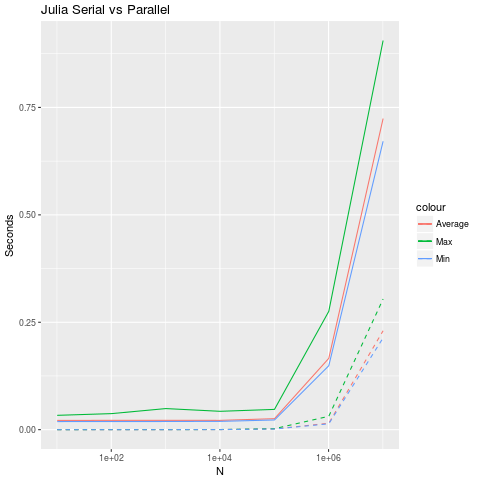
\includegraphics[width=8cm]{plot.png}
\includegraphics[width=8cm]{plot2.png}


As is apparent Table 3, Julia, when compared to the C version of OpenMPI, does very well at lower sample sizes. The high performance at low sample sizes indicates several things. First of all, Julia's parallelization through message passing is better than that of OpenMPI in terms of latency. This comes from the fact that we send more messages with Julia because of the requirement of both function calls and variable requests to be done through message passing, yet we still see a performance on par, if not better than the C implementation of MPI in some cases. However, these tests were performed entirely locally with both implementations. As a result latency over messages is extremely low. Because of the greater volume of messages required by Julia, the performance gain would likely diminish when working on a network cluster, especially if it is not particularly low latency. What is particularly interesting is the across the board better performance ceiling of Julia at low sample sizes. This could be due to less overhead of initialization of nodes for parallelization. Where MPI requires initialization and a variety of variables to be set for each node, Julia only invokes the information required per node from the master node and goes from there.

	Interestingly, Julia appears to struggle when given larger tasks compared to MPI. Due to the very sudden spike in time of the algorithm when compared to MPI, we know that for some reason, the large array size is causing a bottleneck. This is most likely one of two things, either the Message Passing interface of Julia does not have very high throughput, or Julia is having issues performing large-scale array computations. It seems highly unlikely that Julia cannot handle arrays of that large a size given the focus on large array computation by the developers. One issue at hand that could be due to the large array size is vectorization, which causes slowdown in Julia due to extremely efficient for loop implementation.\cite{juliafastcomp} Despite the issue of vectorization though, each of the potentially vectorized commands are in fact specific calls for large arrays. Thus it seems doubtful the Julia developers would write their built in reduction functions without large arrays in mind. Given this information, it seems likely that the implementation of message passing, though low on latency, does not support high throughput. The reasoning for this is with small sample sizes, the latency of the execution as a whole will be most strongly affected by the latency and the throughput can be ignored. However, as you grow, if you have a lower throughput system, the bottleneck will begin to grow your overall delay by a wider margin as happened with Julia vs MPI. 

In order to test whether the bottleneck was due to Julia's Array processing itself, or it's parallelization overhead, we wrote a version of the algorithm in serial in Julia and benchmarked the parallel against serial code. At this point it became entirely clear that the latency was due to throughput issues as the Serial version outperformed Julia in computation time by a wide margin, but performed slightly worse than MPI. Although Julia Performs better than MPI in some cases at low input sizes, it appears to have an overall greater bottleneck due to throughput than MPI. This definitely displays the performance gap of Julia's Parallel utilities when compared to MPI. However, the relative ease of prototyping, could easily make Julia a good choice for parallel processing prototyping.

Finally it should be noted that the Julia code's Just in Time Compiler was actually a major source of bottlenecking. When running code a single time, the compiler would be compiling during the run of the function\cite{juliaparallelslow}, thus for large sample sizes the delay was massive(upwards of 3 seconds for 10 Million sample size). However, if run initially in a function call with a low size, then subsequently timed after the initial compilation, speeds were obtained as can be seen in our speed tests. This also shows the deficiency of Julia when used for smaller scripts as is often done with Python. The JIT compiler will allow for fast prototyping of functions that will be used repeatedly, but will cause major overhead if code is not repeated.

\appendix
\section{Appendix}
\subsection{Source Code}
Credit to Jubobs for Julia formatting in Latex \cite{juliaformatting}.
\fontsize{10}{10}
\begin{lstlisting}
function start(N, cores)

#Start up this many cores
num_cores = Sys.CPU_CORES;

if nprocs()<num_cores
  addprocs(num_cores-1)
end

#A,B - SharedArrays that are global between processes
#A - input array
#B - max value of each bucket
A = SharedArray{Int64}(N);
A = rand(1:32, N);
B = SharedArray{Int64}(num_cores);

#cumul_chunk - Function calculates the cumulative sum of current chunk
#array - input array
#max_array - shared array of max of each chunk
#node_number - process id

@everywhere function cumul_chunk(array, max_array, node_number)
    a = accumulate(+, array)
    max_array[node_number] = maximum(a)
    a
end

#Assumes that the chunk length is divided evenly, specified in MPI version
len = length(A);
per_node = floor(Int, len / num_cores);

#Scatter cumul_chunk for each process to compute with @async
#Gathered in the manager process with fetch
@sync for idx = 1:num_cores
    @async A[(idx - 1)*per_node + 1: per_node*idx] = 
    remotecall_fetch(cumul_chunk,idx,A[(idx - 1)*per_node + 1: per_node*idx],B,idx);	
end

#Apply carryover sums to each bucket
#First chunk doesn't need to do this
#Scattered and gathered the same as above array
@sync for idx = 2:num_cores
    @async A[(idx - 1)*per_node + 1: per_node*idx] = 
    remotecall_fetch( broadcast,idx, +, A[(idx - 1)*per_node + 1: per_node*idx] 
    				,sum(B[1:idx-1]) );	
end

#return A
A
end

#compile
start(10)

#timed run
@time A = start(parse(Int64,ARGS[1]))
\end{lstlisting}
\fontsize{12}{12}
\subsection{Code Highlights}
The code makes use of SharedArrays, which are shared across all processes, so that processes read and write from the same source. The @everywhere macro makes sure that each worker has the necessary function to calculate their cumulative chunks as well as writing to the shared arrays. The @sync and @async macros are used to dispatch the work across each process, but the manager waits until all workers and itself to process each chunk (essentially scatter/gather). The work is dispatched using the low level function call remotecall\_fetch(), which spawns the task at a particular worker and fetches the value when finished. The built-in function accumulate is used to compute the cumulative sum of the chunk (so we don’t reinvent the wheel). The second loop dispatches work to sum the carry over sums in each bucket. The broadcast function is used to apply the sum over every element of the array. The input array is written over by the outputs of the remote calls so it is not immutable.

\subsection{Work Credit}
Alen: Part of Section 1: History and Motivation, Section 2: Structure, Section 5 : Parallelism in Julia, Julia port of Cumulative Sum, and Appendix - Code Highlights  \newline
Colin: Section 3: Speed Comparisons, Section 4: Why is Julia fast?, and part of Section 1: History and Motivation. \newline
Devon: Section 6: Julia vs OpenMPI, Testing scripts, Code Analysis

\printbibliography

\end{document}
